\documentclass{standalone}
\usepackage{tikz}
\usetikzlibrary{patterns, positioning}


\begin{document}
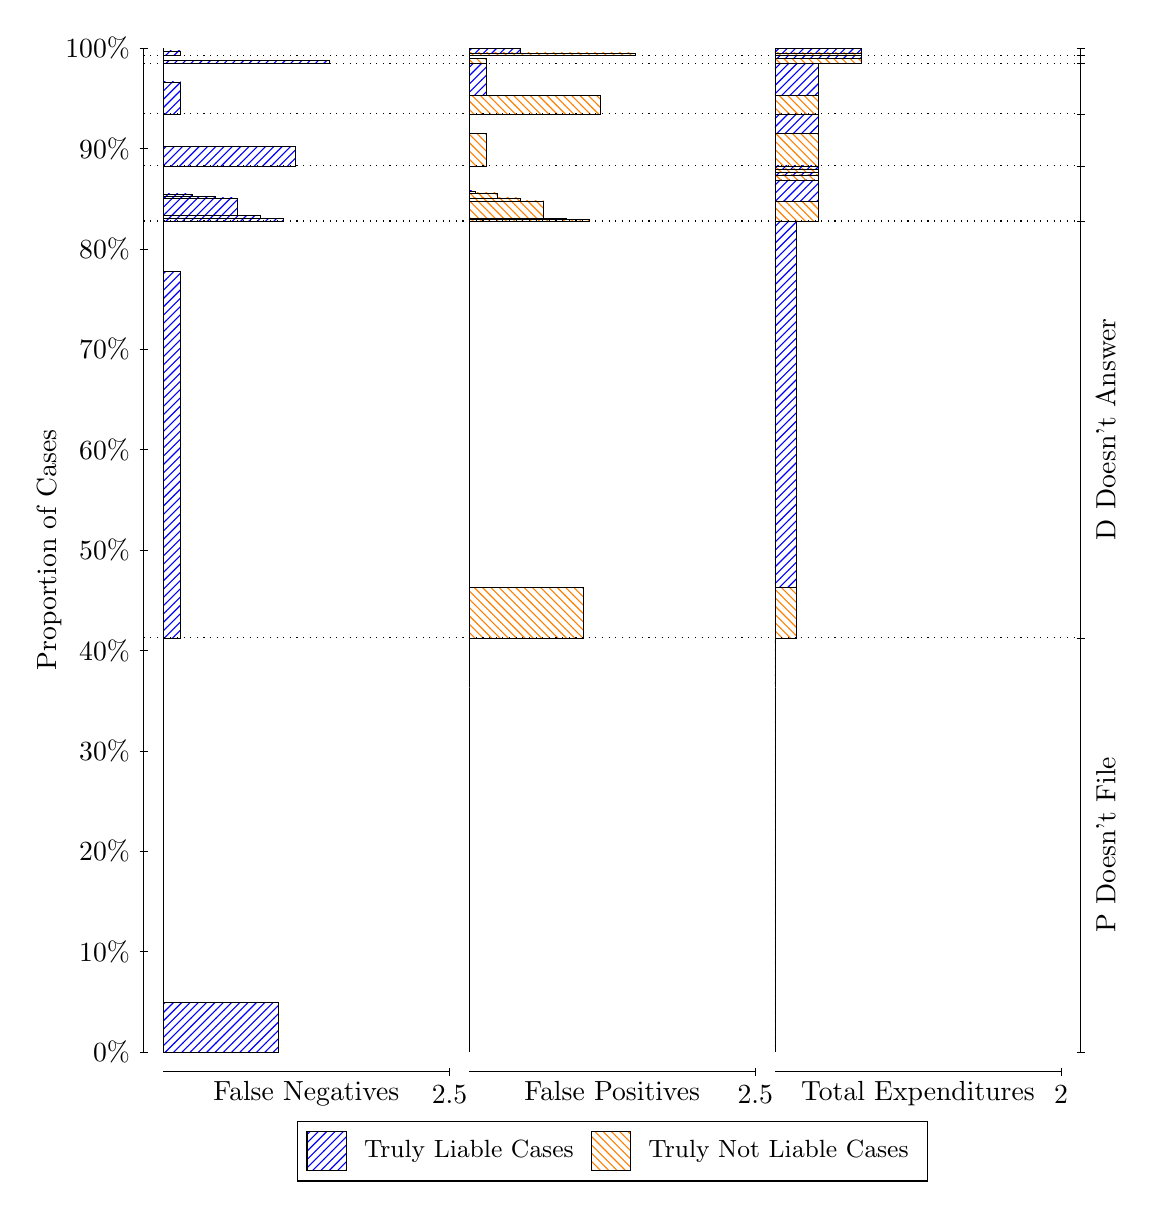
\begin{tikzpicture}
\draw[black, very thin] (1.5,1.75) -- (1.5,14.5);
\node[rotate=90, text=black, anchor=center] at (0.3, 8.125) {Proportion of Cases};
\draw[black, very thin] (1.45,1.75) -- (1.55,1.75);
\node[text=black, anchor=east] at (1.45, 1.75) {0\%};
\draw[black, very thin] (1.45,3.025) -- (1.55,3.025);
\node[text=black, anchor=east] at (1.45, 3.025) {10\%};
\draw[black, very thin] (1.45,4.3) -- (1.55,4.3);
\node[text=black, anchor=east] at (1.45, 4.3) {20\%};
\draw[black, very thin] (1.45,5.575) -- (1.55,5.575);
\node[text=black, anchor=east] at (1.45, 5.575) {30\%};
\draw[black, very thin] (1.45,6.85) -- (1.55,6.85);
\node[text=black, anchor=east] at (1.45, 6.85) {40\%};
\draw[black, very thin] (1.45,8.125) -- (1.55,8.125);
\node[text=black, anchor=east] at (1.45, 8.125) {50\%};
\draw[black, very thin] (1.45,9.4) -- (1.55,9.4);
\node[text=black, anchor=east] at (1.45, 9.4) {60\%};
\draw[black, very thin] (1.45,10.675) -- (1.55,10.675);
\node[text=black, anchor=east] at (1.45, 10.675) {70\%};
\draw[black, very thin] (1.45,11.95) -- (1.55,11.95);
\node[text=black, anchor=east] at (1.45, 11.95) {80\%};
\draw[black, very thin] (1.45,13.225) -- (1.55,13.225);
\node[text=black, anchor=east] at (1.45, 13.225) {90\%};
\draw[black, very thin] (1.45,14.5) -- (1.55,14.5);
\node[text=black, anchor=east] at (1.45, 14.5) {100\%};

\draw[black, very thin] (13.4,1.75) -- (13.4,14.5);
\draw[black, very thin] (13.35,1.75) -- (13.45,1.75);
\node[anchor=west] at (13.35, 1.75) {};
\draw[black, very thin] (13.35,7.01) -- (13.45,7.01);
\node[anchor=west] at (13.35, 7.01) {};
\draw[black, very thin] (13.35,12.303) -- (13.45,12.303);
\node[anchor=west] at (13.35, 12.303) {};
\draw[black, very thin] (13.35,13.003) -- (13.45,13.003);
\node[anchor=west] at (13.35, 13.003) {};
\draw[black, very thin] (13.35,13.663) -- (13.45,13.663);
\node[anchor=west] at (13.35, 13.663) {};
\draw[black, very thin] (13.35,14.309) -- (13.45,14.309);
\node[anchor=west] at (13.35, 14.309) {};
\draw[black, very thin] (13.35,14.403) -- (13.45,14.403);
\node[anchor=west] at (13.35, 14.403) {};
\draw[black, very thin] (13.35,14.5) -- (13.45,14.5);
\node[anchor=west] at (13.35, 14.5) {};

\draw[black, very thin, pattern color=blue, pattern=north east lines] (1.75,1.75) rectangle (3.2033,2.3828);
\draw[black, very thin, pattern color=orange, pattern=north west lines] (1.75,2.3828) rectangle (1.75,7.01);
\draw[black, very thin, pattern color=blue, pattern=north east lines] (1.75,7.01) rectangle (1.968,11.66);
\draw[black, very thin, pattern color=orange, pattern=north west lines] (1.75,11.66) rectangle (1.75,12.303);
\draw[black, very thin, pattern color=blue, pattern=north east lines] (1.75,12.303) rectangle (3.276,12.34);
\draw[black, very thin, pattern color=blue, pattern=north east lines] (1.75,12.34) rectangle (3.1307,12.341);
\draw[black, very thin, pattern color=blue, pattern=north east lines] (1.75,12.341) rectangle (2.9853,12.379);
\draw[black, very thin, pattern color=blue, pattern=north east lines] (1.75,12.379) rectangle (2.6947,12.596);
\draw[black, very thin, pattern color=blue, pattern=north east lines] (1.75,12.596) rectangle (2.404,12.617);
\draw[black, very thin, pattern color=blue, pattern=north east lines] (1.75,12.617) rectangle (2.2587,12.619);
\draw[black, very thin, pattern color=blue, pattern=north east lines] (1.75,12.619) rectangle (2.1133,12.647);
\draw[black, very thin, pattern color=orange, pattern=north west lines] (1.75,12.647) rectangle (1.75,13.003);
\draw[black, very thin, pattern color=blue, pattern=north east lines] (1.75,13.003) rectangle (3.4213,13.248);
\draw[black, very thin, pattern color=orange, pattern=north west lines] (1.75,13.248) rectangle (1.75,13.663);
\draw[black, very thin, pattern color=blue, pattern=north east lines] (1.75,13.663) rectangle (1.968,14.07);
\draw[black, very thin, pattern color=orange, pattern=north west lines] (1.75,14.07) rectangle (1.75,14.309);
\draw[black, very thin, pattern color=blue, pattern=north east lines] (1.75,14.309) rectangle (3.8573,14.344);
\draw[black, very thin, pattern color=orange, pattern=north west lines] (1.75,14.344) rectangle (1.75,14.403);
\draw[black, very thin, pattern color=blue, pattern=north east lines] (1.75,14.403) rectangle (1.968,14.464);
\draw[black, very thin, pattern color=orange, pattern=north west lines] (1.75,14.464) rectangle (1.75,14.5);
\draw[black, very thin, pattern color=orange, pattern=north west lines] (5.6333,1.75) rectangle (5.6333,6.3773);
\draw[black, very thin, pattern color=blue, pattern=north east lines] (5.6333,6.3773) rectangle (5.6333,7.01);
\draw[black, very thin, pattern color=orange, pattern=north west lines] (5.6333,7.01) rectangle (7.0867,7.6533);
\draw[black, very thin, pattern color=blue, pattern=north east lines] (5.6333,7.6533) rectangle (5.6333,12.303);
\draw[black, very thin, pattern color=orange, pattern=north west lines] (5.6333,12.303) rectangle (7.1593,12.319);
\draw[black, very thin, pattern color=orange, pattern=north west lines] (5.6333,12.319) rectangle (7.014,12.321);
\draw[black, very thin, pattern color=orange, pattern=north west lines] (5.6333,12.321) rectangle (6.8687,12.341);
\draw[black, very thin, pattern color=orange, pattern=north west lines] (5.6333,12.341) rectangle (6.578,12.558);
\draw[black, very thin, pattern color=orange, pattern=north west lines] (5.6333,12.558) rectangle (6.2873,12.597);
\draw[black, very thin, pattern color=orange, pattern=north west lines] (5.6333,12.597) rectangle (6.142,12.597);
\draw[black, very thin, pattern color=orange, pattern=north west lines] (5.6333,12.597) rectangle (5.9967,12.659);
\draw[black, very thin, pattern color=blue, pattern=north east lines] (5.6333,12.659) rectangle (5.706,12.686);
\draw[black, very thin, pattern color=blue, pattern=north east lines] (5.6333,12.686) rectangle (5.6333,13.003);
\draw[black, very thin, pattern color=orange, pattern=north west lines] (5.6333,13.003) rectangle (5.8513,13.418);
\draw[black, very thin, pattern color=blue, pattern=north east lines] (5.6333,13.418) rectangle (5.6333,13.663);
\draw[black, very thin, pattern color=orange, pattern=north west lines] (5.6333,13.663) rectangle (7.3047,13.902);
\draw[black, very thin, pattern color=blue, pattern=north east lines] (5.6333,13.902) rectangle (5.8513,14.309);
\draw[black, very thin, pattern color=orange, pattern=north west lines] (5.6333,14.309) rectangle (5.8513,14.367);
\draw[black, very thin, pattern color=blue, pattern=north east lines] (5.6333,14.367) rectangle (5.6333,14.403);
\draw[black, very thin, pattern color=orange, pattern=north west lines] (5.6333,14.403) rectangle (7.7407,14.439);
\draw[black, very thin, pattern color=blue, pattern=north east lines] (5.6333,14.439) rectangle (6.2873,14.5);
\draw[black, very thin, pattern color=orange, pattern=north west lines] (9.5167,1.75) rectangle (9.5167,6.3773);
\draw[black, very thin, pattern color=blue, pattern=north east lines] (9.5167,6.3773) rectangle (9.5167,7.01);
\draw[black, very thin, pattern color=orange, pattern=north west lines] (9.5167,7.01) rectangle (9.7892,7.6533);
\draw[black, very thin, pattern color=blue, pattern=north east lines] (9.5167,7.6533) rectangle (9.7892,12.303);
\draw[black, very thin, pattern color=orange, pattern=north west lines] (9.5167,12.303) rectangle (10.062,12.558);
\draw[black, very thin, pattern color=blue, pattern=north east lines] (9.5167,12.558) rectangle (10.062,12.826);
\draw[black, very thin, pattern color=orange, pattern=north west lines] (9.5167,12.826) rectangle (10.062,12.888);
\draw[black, very thin, pattern color=blue, pattern=north east lines] (9.5167,12.888) rectangle (10.062,12.925);
\draw[black, very thin, pattern color=orange, pattern=north west lines] (9.5167,12.925) rectangle (10.062,12.964);
\draw[black, very thin, pattern color=blue, pattern=north east lines] (9.5167,12.964) rectangle (10.062,13.003);
\draw[black, very thin, pattern color=orange, pattern=north west lines] (9.5167,13.003) rectangle (10.062,13.418);
\draw[black, very thin, pattern color=blue, pattern=north east lines] (9.5167,13.418) rectangle (10.062,13.663);
\draw[black, very thin, pattern color=orange, pattern=north west lines] (9.5167,13.663) rectangle (10.062,13.902);
\draw[black, very thin, pattern color=blue, pattern=north east lines] (9.5167,13.902) rectangle (10.062,14.309);
\draw[black, very thin, pattern color=orange, pattern=north west lines] (9.5167,14.309) rectangle (10.607,14.367);
\draw[black, very thin, pattern color=blue, pattern=north east lines] (9.5167,14.367) rectangle (10.607,14.403);
\draw[black, very thin, pattern color=orange, pattern=north west lines] (9.5167,14.403) rectangle (10.607,14.439);
\draw[black, very thin, pattern color=blue, pattern=north east lines] (9.5167,14.439) rectangle (10.607,14.5);
\draw[black, dotted] (1.5,7.01) -- (13.4,7.01);
\draw[black, dotted] (1.5,12.303) -- (13.4,12.303);
\draw[black, dotted] (1.5,13.003) -- (13.4,13.003);
\draw[black, dotted] (1.5,13.663) -- (13.4,13.663);
\draw[black, dotted] (1.5,14.309) -- (13.4,14.309);
\draw[black, dotted] (1.5,14.403) -- (13.4,14.403);
\draw[black, very thin] (1.75,1.5) -- (5.3833,1.5);
\node[text=black, anchor=north] at (3.5667, 1.5) {False Negatives};
\draw[black, very thin] (5.3833,1.45) -- (5.3833,1.55);
\node[text=black, anchor=north] at (5.3833, 1.45) {2.5};

\draw[black, very thin] (5.6333,1.5) -- (9.2667,1.5);
\node[text=black, anchor=north] at (7.45, 1.5) {False Positives};
\draw[black, very thin] (9.2667,1.45) -- (9.2667,1.55);
\node[text=black, anchor=north] at (9.2667, 1.45) {2.5};

\draw[black, very thin] (9.5167,1.5) -- (13.15,1.5);
\node[text=black, anchor=north] at (11.333, 1.5) {Total Expenditures};
\draw[black, very thin] (13.15,1.45) -- (13.15,1.55);
\node[text=black, anchor=north] at (13.15, 1.45) {2};

\node[text=black, centered, rotate=90] at (13.72, 4.38) {P Doesn't File};
\node[text=black, centered, rotate=90] at (13.72, 9.6565) {D Doesn't Answer};






\draw (7.449999999999999,1.5) node[draw=none] (baseCoordinate) {};
\begin{scope}[align=center]
        \matrix[scale=0.5, draw=black, below=0.5cm of baseCoordinate, nodes={draw}, column sep=0.1cm]{
            \node[rectangle, draw, minimum width=0.5cm, minimum height=0.5cm, pattern color=blue, pattern=north east lines] {}; &
            \node[draw=none, font=\small, text=black] (B) {Truly Liable Cases}; &
            \node[rectangle, draw, minimum width=0.5cm, minimum height=0.5cm, pattern color=orange, pattern=north west lines] {}; &
            \node[draw=none, font=\small, text=black] (B) {Truly Not Liable Cases}; \\
            };
\end{scope}

\end{tikzpicture}
\end{document}